%----------------------------------------------------------------------------------------
%	ESTADO DEL ARTE (20-25 hojas)
%----------------------------------------------------------------------------------------

\pagestyle{empty}
\chapter {Estado del Arte}

La realidad virtual actualmente abarca muchas areas y se puede interactuar con ella de muchas formas. La forma más común y en la cual se va a centrar este documento es en la representación de imágenes mediante un casco o gafas de realidad virtual.


%\section{Fotografía y vídeo}
%La fotografía y el vídeo en realidad virtual es un campo muy amplio en el que se pueden encontrar diferentes maneras guardar y reproducir la información.

%\subsection{Estereoscopía}
%La estereoscopía es el factor más importante en contenido multimedia. En el caso de las imágenes consiste en tener dos imágenes que representan la misma escena desde dos puntos cercanos que representan los ojos. Cada una de estas imágenes se reproducen en una de las pantallas de las gafas, de tal manera que el

%\subsection{Ángulos de proyección}
%Dentro de fotografía

\section{Mapas de profundidad}
Debido a la cantidad de técnicas que utilizan mapas de profundidad es interesante explicar en que consisten. 

Los mapas de profundidad son imagenes que en cada pixel se encuentra codificada la profundidad de la foto en ese punto. Generalmente se utiliza una escala de grises o de rojos aunque se pueden recurrir a métodos más complejos.\cite{Josh6DoFUnity}

En el caso de la escala de grises (\ref{fig:depthmap-example}), los tonos más oscuros representan elementos en el fondo de la imagen, mientras que los tonos mas claro representan elementos más cercanos.
\begin{figure}[h]
  \centering
  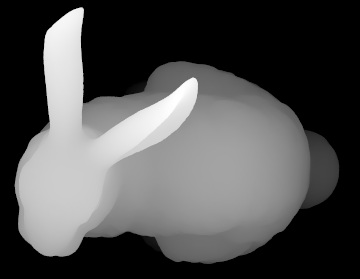
\includegraphics[width=0.7\textwidth]{depthmap-example}
  \caption{Ejemplo de mapa de profundidad cenital}
  \label{fig:depthmap-example}
\end{figure}

En el caso de una imagen generada por ordenador, es fácil obetener un buen mapa de profundidad. Sin embargo en el caso de las imágenes captadas por cámaras reales, existe la posibilidad de que la cámara esté preparada y también obtenga la profundidad o en caso contrario habría que aplicar algoritmos que calculen la profundidad en cada píxel. Estos algoritmos no son perfectos y en ocasiones el mapa obtenido tiene ruido y puede afectar a las técnicas que lo usen.

\section{Project Sidewinder}
Adobe presento en 2017 \cite{SidewinderAdobe} una demo que utilizaba un depthmap de manera muy sencilla para permitir seis grados de libertad dentro de un video 360º. No proporcionan mucha información ya que es una prueba de concepto.

El desplazamiento punto a punto parece correcto pero se ve una distorsión en los bordes probablemente debido al estado temprano del proyecto.

\section{Nube de puntos}
Esta técnica consiste en crear un punto en el espacio por cada pixel de la foto o el vídeo y utilizar la imagen y su mapa de profundidad para seleccionar el color y el desplazamiento del punto en el espacio. \cite{UploadVR}

\begin{figure}[h]
  \centering
  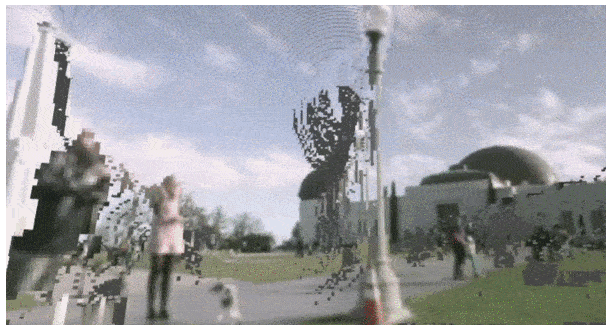
\includegraphics[width=0.8\textwidth]{pointcloud-example}
  \caption{Ejemplo de nube de puntos}
  \label{fig:pointcloud-example}
\end{figure}

Esta implementación por contra provoca que aparezcan muchos huecos como se puede ver en \ref{fig:depthmap-example} y generalmente se suele acompañar la implementación con una selección del tamaño del punto como muestra \cite{Josh6DoFUnity} para ver una imagen más sólida.

Otro de los problemas que tiene esta técnica es la cantidad de puntos que deben ser tratados, ya que una resolución QHD (2560x1440) requiere cuatro millones de puntos siendo la resolución recomendada actualmente es 4K.


\section{Cámara y herramientas de realidad virtual de OTOY y Facebook}

En el F8 de 2017 en Los Ángeles \textit{OTOY} y \textit{Facebook} presentaron una colaboración para producir vídeo 360º volumétrico e interactivo a un precio asequible \cite{OtoyVR}. No hay noticias de 2018 por lo que puede que esté abandonado.

La colaboración consistía en una cámara 360º especializada y una serie de herramientas para procesar el contenido y visualizarlo. El procedimiento implica subir el contenido a la nube de OTOY para procesarlo y así reconstruir la escena como una malla tridimensional. 

La calidad presentada en las demos era buena con poca distorsión aunque el desplazamiento que presentaban era pequeño.

\section{Seis Grados de libertad con Fotogrametría}
Una de las formas de conseguir seis grados de libertad es reconstruir la escena mediante fotogrametría como muestra \textit{Facebook} en \cite{FBCasual3DCapture} para procesar la imagen y obtener una malla que pueda ser mostrada usando técnicas convencionales.

\begin{figure}[h]
  \centering
	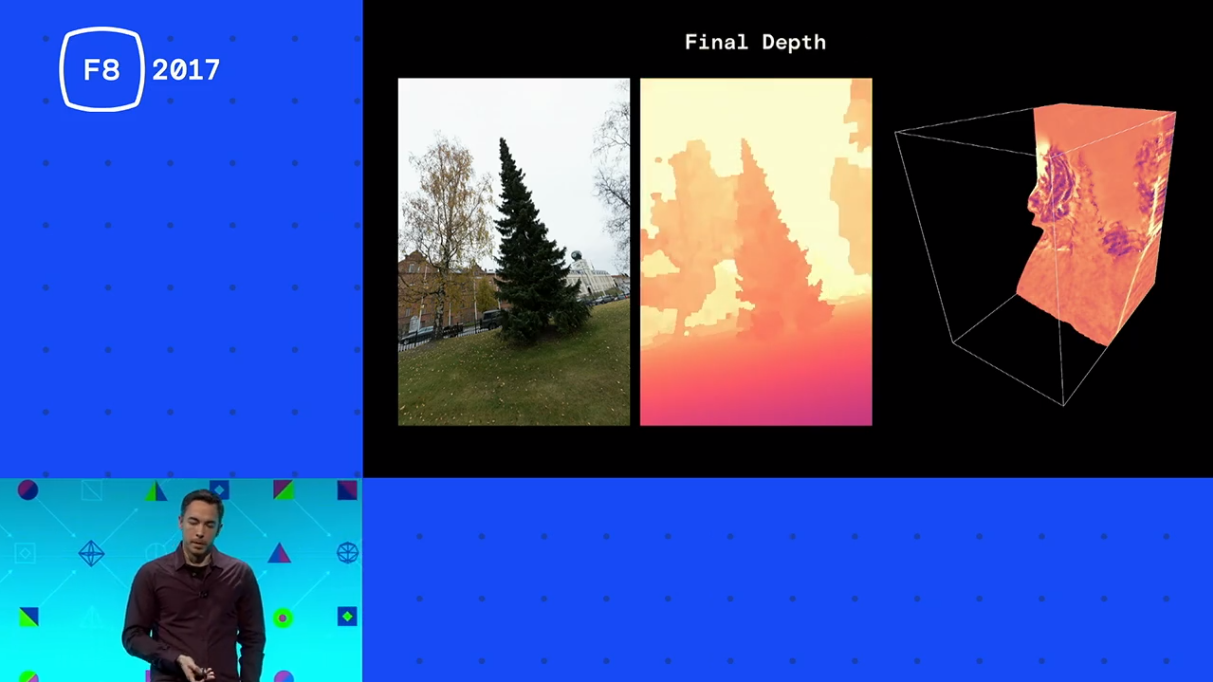
\includegraphics[width=\linewidth]{FB/fbdepthmap}
  \caption{Conferencia mostrando un mapa de profundidad de limite inferior}
  \label{fig:fbLBdepthmap-example}
\end{figure}

Este procedimiento utiliza una técnica nueva que han llamado mapa de profundidad de limite inferior \ref{fig:depthmap-example} que la profundidad de cada pixel debe ser estrictamente mayor que en el depthmap normal. Crear este mapa de profundidad le ayuda al ensamblado de las imágenes para crear la imágen final 360º. Además mezclando el mapa de profundidad con otros algoritmos son capaces de obtener un mapa de normales bastante preciso. \ref{fig:fbnormalmapcorrected-example}

\begin{figure}[h]
\centering
\begin{subfigure}{.47\linewidth}
	\centering
	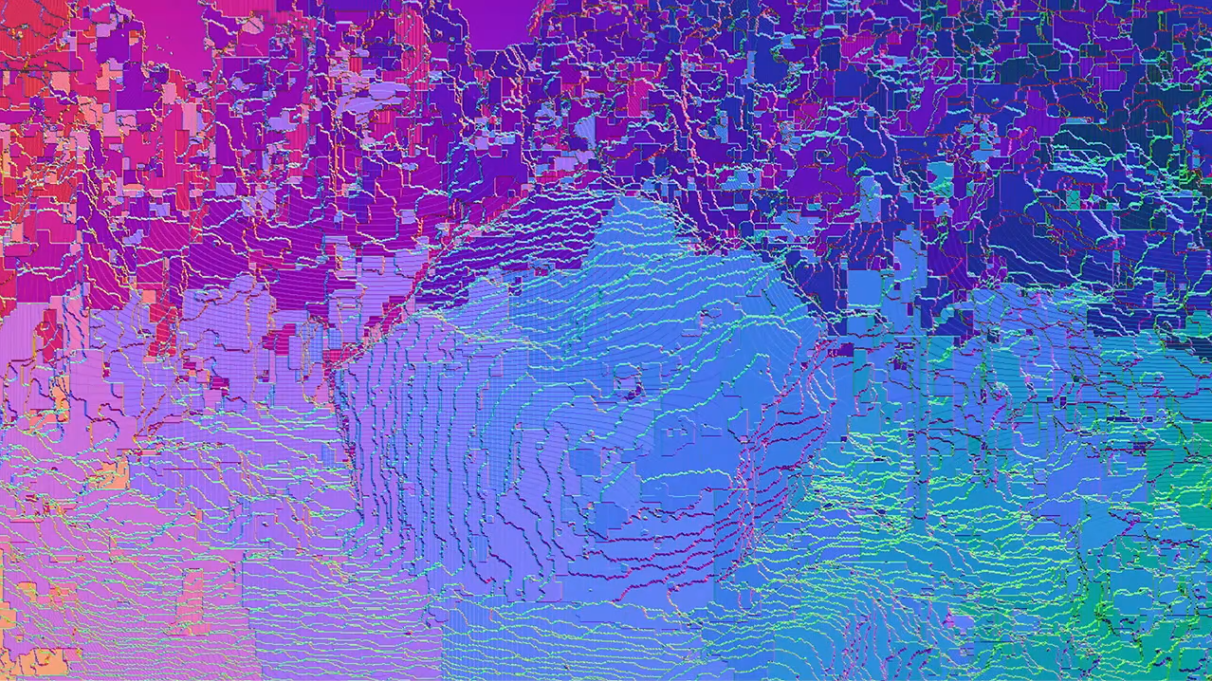
\includegraphics[width=\linewidth]{FB/fbnormalartifacts}
  \caption{Conferencia mostrando los artefactos que obtienen}
  \label{fig:fbnormalmapartifacts-example}
\end{subfigure}%
\hspace{.05\linewidth}
\begin{subfigure}{.47\linewidth}
	\centering
	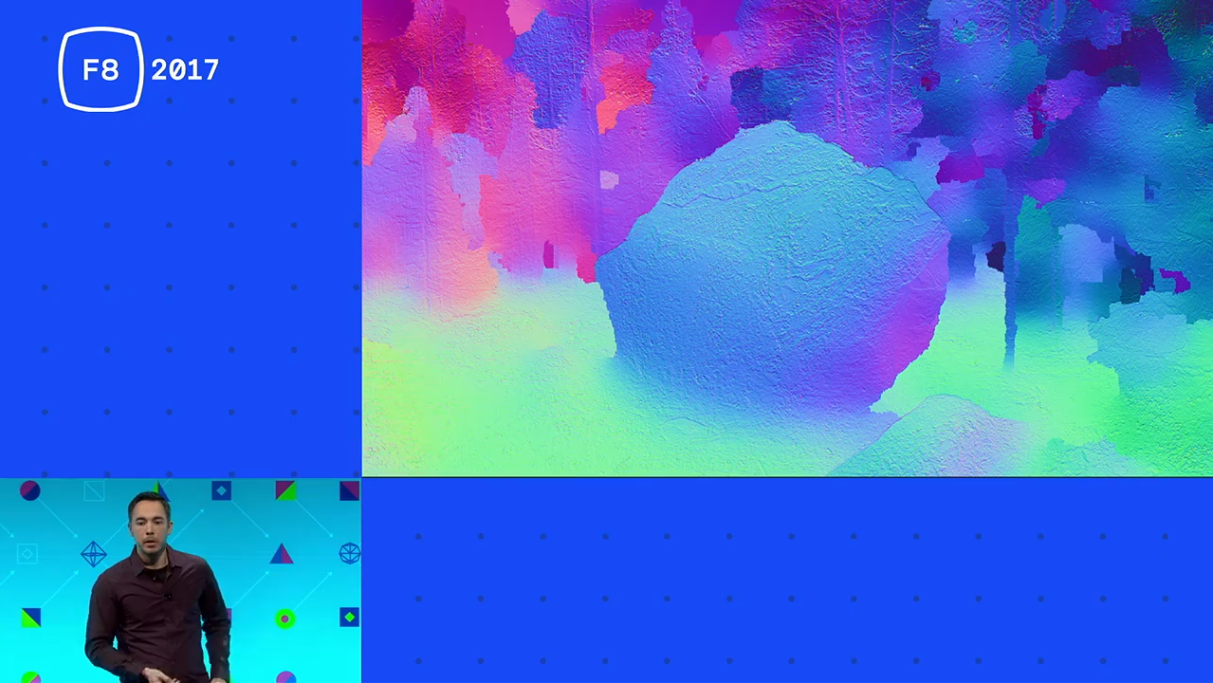
\includegraphics[width=\linewidth]{FB/fbnormalmap}
  \caption{Conferencia mostrando los artefactos arreglados}
  \label{fig:fbnormalmapcorrected-example}
\end{subfigure}
\end{figure}


Finalmente crean la malla a partir de una nube de puntos. Esta malla como veremos en otras técnicas, tiene agujeros detrás de los objetos que no pueden ser rellenados por falta de información. En este caso optan por difuminar de manera sutil las zonas desconocidas dando un buen resultado.

Todo esto lo aprovechan para poder generar un entorno tridimensional con el que poder interactuar y lo ejemplifican jugando con la iluminación \ref{fig:fblighting-example} o incluso inundando la escena \ref{fig:fbflooding-example}.

\begin{figure}[h]
\centering
\begin{subfigure}{.47\linewidth}
	\centering
	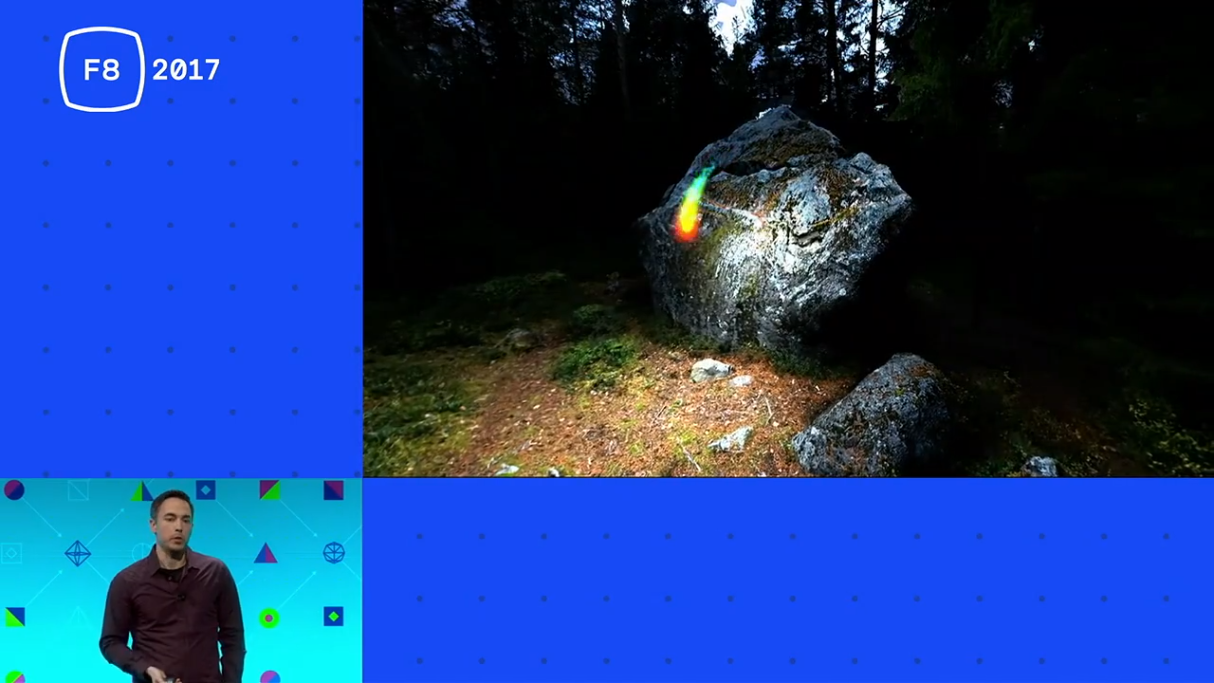
\includegraphics[width=\linewidth]{FB/fblighting}
  \caption{Conferencia mostrando la malla iluminada}
  \label{fig:fblighting-example}
\end{subfigure}%
\hspace{.05\linewidth}
\begin{subfigure}{.47\linewidth}
	\centering
	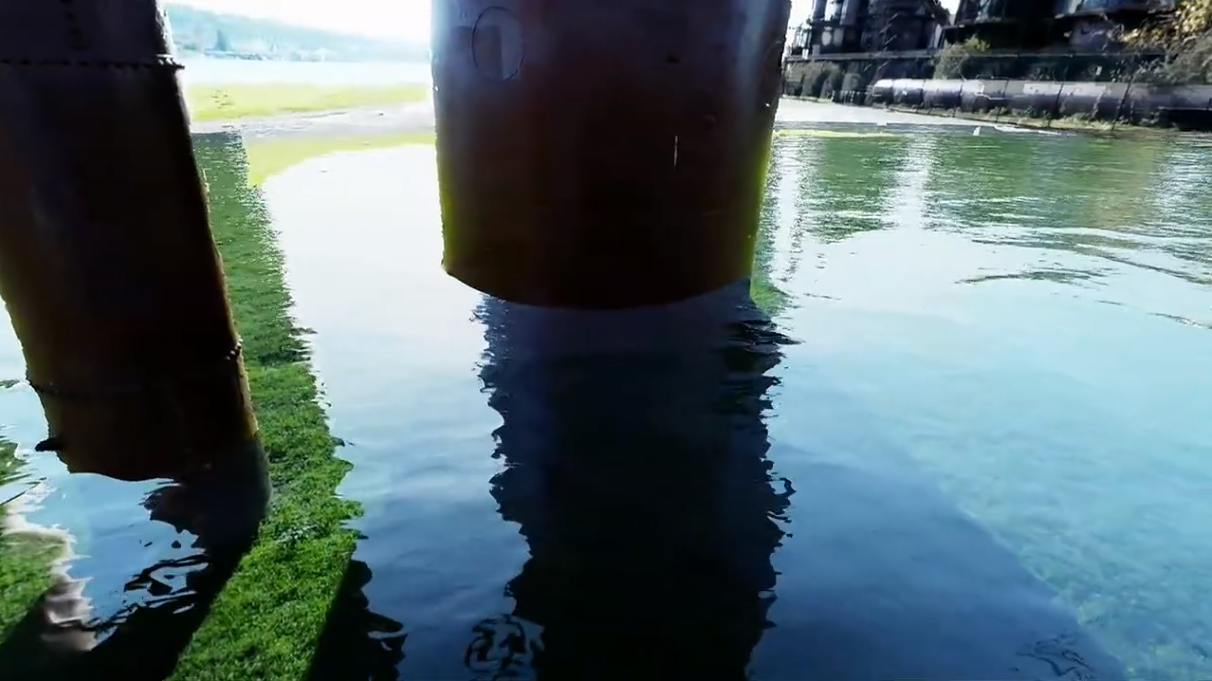
\includegraphics[width=\linewidth]{FB/fbflooding}
  \caption{Conferencia mostrando un escenario inundándose}
  \label{fig:fbflooding-example}
\end{subfigure}
\end{figure}

Una de las limitaciones que tiene este método es que está diseñado para fotografía en 360º y no se menciona en ningún momento al vídeo 360º por lo que se puede deducir que no está preparado. Por otro lado este tipo de procesado de imágenes requiere una cantidad grande de tiempo.

\section{``Welcome to Lightfields''}
Una compañía llamada Lytro creo un sistema que llamo campos de luz o Lightfields \cite{LytroLightfields} por su similitud con el concepto físico. Más tarde Google se interesó por la compañía comprando algunas de sus patentes e incorporando empleados a su plantilla.

\textit{Google} continuó el proyecto \cite{GoogleLightfields} y construyó un soporte que permite hacer fotografías de una escena desde puntos situados en una esfera.

\begin{figure}[h]
  \centering
	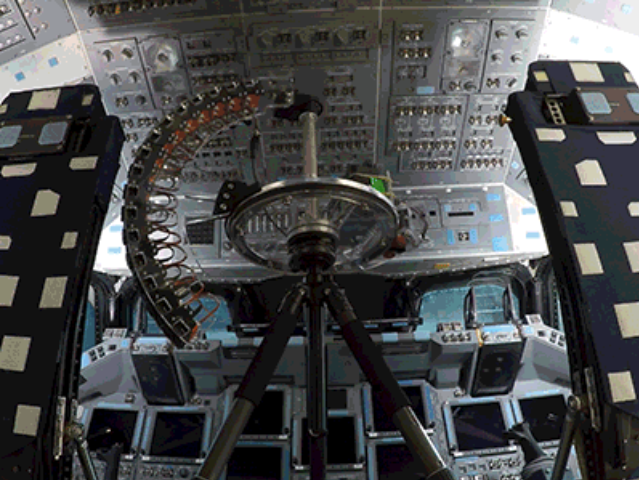
\includegraphics[width=\linewidth]{lightfields-camera}
  \caption{Prototipo haciendo una captura del interior de una cabina.}
  \label{fig:lightfields-camera}
\end{figure}

A partir de todas las fotos recuperadas se calcula la imagen correspondiente en función de la posición del usuario haciendo una interpolación entre diferentes imágenes, eso hace que se recupere una imagen muy fiel a lo que se vería en la realidad. 

\begin{figure}[h]
  \centering
	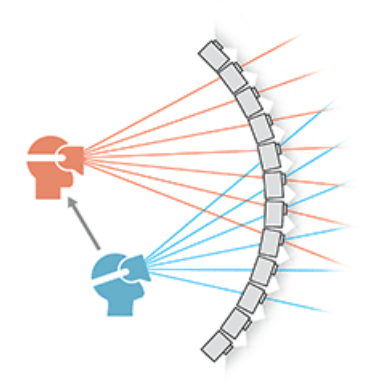
\includegraphics[width=0.5\linewidth]{lightfields-schema}
  \caption{Esquema de funcionamiento de los lightfields.}
  \label{fig:lightfields-schema}
\end{figure}

Además esto tiene una implicación que no había sido contemplada hasta ahora que son las superficies especulares. Estas superficies en el resto de técnicas se podían ver con reflejo o no, pero nunca respondería a la posición del usuario. La interpolación de imágenes hace que los espejos reflejen algo diferente en cada posición de la cabeza.

Esta técnica para fotografía es probablemente la mejor en cuanto a calidad de imagen pero sin embargo no se puede utilizar en vídeo debido al tiempo que se tarda en capturar un sólo fotograma. Tampoco permite alterar la luz como se mostraba en la demo de \textit{Facebook}.











